% Manuscript source. Plain-language note: this is the text of the paper, laid out as a
% two-column journal article. Every result is a macro (for example \LMest) defined in
% numbers.tex, which code/05_manuscript.py writes from stats.json. Build with:
%   python3 code/05_manuscript.py --final
\documentclass[10pt,twocolumn,letterpaper]{article}
\usepackage[letterpaper,top=0.9in,bottom=0.9in,left=0.72in,right=0.72in,columnsep=0.3in,headsep=0.25in]{geometry}

\usepackage{amsmath,graphicx,booktabs,xcolor,enumitem,microtype,fancyhdr,titlesec,caption}
\usepackage[authoryear,round,sort]{natbib}
\definecolor{linkblue}{rgb}{0.16,0.29,0.66}
\usepackage[colorlinks=true,linkcolor=linkblue,citecolor=linkblue,urlcolor=linkblue]{hyperref}
\usepackage{orcidlink}
% Generated by code/05_manuscript.py from paper/stats.json. Do not edit by hand.
\newcommand{\Nrand}{1{,}019}
\newcommand{\Nact}{516}
\newcommand{\Nlec}{503}
\newcommand{\Nstay}{811}
\newcommand{\NstayAct}{417}
\newcommand{\NstayLec}{394}
\newcommand{\Nleft}{208}
\newcommand{\StayRateAct}{80.8\%}
\newcommand{\StayRateLec}{78.3\%}
\newcommand{\StayP}{$p = .325$}
\newcommand{\Nsections}{32}
\newcommand{\Nslots}{16}
\newcommand{\Ninstr}{19}
\newcommand{\NinstrAct}{7}
\newcommand{\NinstrLec}{12}
\newcommand{\Nclusters}{32}
\newcommand{\Ndf}{31}
\newcommand{\LMnAct}{376}
\newcommand{\LMnLec}{310}
\newcommand{\LMmeanAct}{63.5}
\newcommand{\LMmeanLec}{47.7}
\newcommand{\LMsdAct}{19.8}
\newcommand{\LMsdLec}{21.0}
\newcommand{\LMest}{15.8}
\newcommand{\LMlo}{11.8}
\newcommand{\LMhi}{19.8}
\newcommand{\LMp}{$p < .001$}
\newcommand{\LMadj}{16.3}
\newcommand{\LMadjLo}{12.8}
\newcommand{\LMadjHi}{19.7}
\newcommand{\Gval}{0.77}
\newcommand{\Glo}{0.62}
\newcommand{\Ghi}{0.93}
\newcommand{\PairsFav}{14}
\newcommand{\PairsN}{16}
\newcommand{\PairsMean}{16.1}
\newcommand{\PairsPexact}{$p < .001$}
\newcommand{\PairsPt}{$p < .001$}
\newcommand{\LeeLo}{11.7}
\newcommand{\LeeHi}{20.7}
\newcommand{\LeeGlo}{0.57}
\newcommand{\LeeGhi}{1.02}
\newcommand{\LeeTrim}{12.7\%}
\newcommand{\MissAct}{9.8\%}
\newcommand{\MissLec}{21.3\%}
\newcommand{\PassAct}{80.3\%}
\newcommand{\PassLec}{68.5\%}
\newcommand{\PassEst}{11.7}
\newcommand{\PassLo}{6.4}
\newcommand{\PassHi}{17.1}
\newcommand{\PassP}{$p < .001$}
\newcommand{\PassAdj}{11.9}
\newcommand{\PassAdjLo}{6.8}
\newcommand{\PassAdjHi}{17.0}
\newcommand{\PassPairsFav}{12}
\newcommand{\PassPairsMean}{11.6}
\newcommand{\PassPairsPexact}{$p = .008$}
\newcommand{\DFWAct}{19.7\%}
\newcommand{\DFWLec}{31.5\%}
\newcommand{\DFWRed}{37.5\%}
\newcommand{\PerHundred}{12}
\newcommand{\PrepAct}{65.2}
\newcommand{\PrepLec}{65.9}
\newcommand{\PrepP}{$p = .356$}
\newcommand{\PrepNoScoreLec}{63.3}
\newcommand{\PrepScoreLec}{66.7}
\newcommand{\SubLMmin}{15.4}
\newcommand{\SubLMmax}{17.3}
\newcommand{\SubPassHisp}{14.5}
\newcommand{\SubPassTransfer}{16.7}
\newcommand{\BlackPassAct}{70.0\%}
\newcommand{\BlackPassLec}{51.9\%}
\newcommand{\Nblack}{104}
\newcommand{\MinInterP}{0.16}
\newcommand{\ShareHisp}{71.3\%}
\newcommand{\AuthorName}{Faith Oluwafunmitan Esan}
\newcommand{\AuthorOrcid}{0009-0001-3694-157X}
\newcommand{\AuthorEmail}{faithesan14@gmail.com}
\newcommand{\AuthorAffil}{Independent Researcher, Laramie, Wyoming, USA}
\newcommand{\RepoURL}{https://github.com/faithesan-hub/calculus-active-learning}
\newif\ifdraftcopy\draftcopyfalse


% ---- journal-style layout ----
\setlength{\parindent}{1em}
\setlength{\parskip}{0pt}
\renewcommand{\thesection}{\arabic{section}}
\renewcommand{\thesubsection}{\thesection.\arabic{subsection}}
\titleformat{\section}{\normalfont\centering}{\thesection.}{0.5em}{\MakeUppercase}
\titlespacing*{\section}{0pt}{12pt plus 2pt}{5pt}
\titleformat{\subsection}{\normalfont\itshape\centering}{\thesubsection.}{0.5em}{}
\titlespacing*{\subsection}{0pt}{8pt plus 2pt}{4pt}
\captionsetup{font=small,labelfont=bf,labelsep=period,justification=justified,singlelinecheck=true}
\captionsetup[table]{labelfont={sc},font=small,justification=centering,labelsep=period,skip=4pt}
\newcommand{\tablecomments}[1]{\par\vspace{3pt}\parbox{0.96\textwidth}{\footnotesize\textsc{Note}---#1}}
\newcommand{\nodata}{\ldots}
\pagestyle{fancy}\fancyhf{}
\fancyhead[LE,RO]{\small\thepage}
\renewcommand{\headrulewidth}{0pt}
\fancypagestyle{plain}{\fancyhf{}\renewcommand{\headrulewidth}{0pt}}
\setlist[itemize]{leftmargin=1.6em,itemsep=4pt}
\bibliographystyle{plainnat}
\raggedbottom
\setcounter{dbltopnumber}{2}
\renewcommand{\dbltopfraction}{0.85}
\renewcommand{\dblfloatpagefraction}{0.8}
\renewcommand{\textfraction}{0.08}

\begin{document}
\twocolumn[
\begin{@twocolumnfalse}
\vspace*{-0.35in}
{\footnotesize
\ifdraftcopy\textsc{Draft version, not for circulation}\else\textsc{Preprint version October 10, 2026}\fi\\
Typeset using \LaTeX\ \textbf{twocolumn} journal style\par}
\vspace{0.35in}
\begin{center}
{\large\bfseries Active Learning in First-Semester Calculus: An Open Re-analysis of a\\[2pt] Randomized Trial at a Hispanic-Serving Institution\par}
\vspace{8pt}
\href{https://orcid.org/\AuthorOrcid}{\textsc{\AuthorName}}\,\orcidlink{\AuthorOrcid}$^{1,*}$\par
\vspace{4pt}
{\small $^{1}$\textit{\AuthorAffil}\par}
\vspace{12pt}
ABSTRACT\par
\vspace{4pt}
\begin{minipage}{0.84\textwidth}
\setlength{\parindent}{1em}\indent
Active learning is widely recommended in college mathematics, but much of the evidence comes from studies whose data cannot be checked. We re-analyze the openly shared data from a pragmatic trial in which \Nrand\ first-semester calculus students at a large Hispanic-Serving Institution were randomly allocated to active-learning (Modeling Practices in Calculus) or lecture sections across \Nsections\ sections and \Nslots\ registration time slots \citep{kramer2023}. Among the \Nstay\ students who remained in their assigned section, active-learning students scored \LMest\ points higher on a common 0--100 end-of-term learning measure (95\% CI \LMlo\ to \LMhi; Hedges' $g = \Gval$) and were \PassEst\ percentage points more likely to pass with a C or better (\PassAct\ vs.\ \PassLec; 95\% CI \PassLo\ to \PassHi). The active section outperformed its lecture counterpart on the learning measure in \PairsFav\ of \PairsN\ time slots. Because lecture students were more likely to lack a learning score, we estimate Lee bounds; the learning gain remains at least \LeeLo\ points. Effects are similar across gender, ethnicity, transfer status, and prior preparation. All code and derived data are public so that others can reproduce, challenge, and extend these results.
\par\vspace{6pt}
\noindent\textit{Keywords:} active learning --- cooperative learning --- calculus --- randomized trial --- open science --- Hispanic-Serving Institutions --- replication
\end{minipage}
\end{center}
\vspace{14pt}
\end{@twocolumnfalse}
]
{\let\thefootnote\relax\footnotetext{$^*$ E-mail: \href{mailto:\AuthorEmail}{\AuthorEmail}}}

\section{Introduction}

First-semester calculus is a gateway to nearly every science, engineering, and health degree. Large national studies have documented that many students who begin calculus do not succeed in it, and that a poor calculus experience is associated with leaving STEM majors \citep{bressoud2015}. Teaching that asks students to work problems in class, often in small groups, has been proposed as one remedy.

Meta-analyses support this view across STEM. \citet{springer1999} found benefits of small-group learning in undergraduate science and mathematics. \citet{freeman2014} synthesized 225 studies and found higher examination scores and lower failure rates under active learning, and \citet{theobald2020} found that active learning narrowed achievement gaps for underrepresented students. \citet{laursen2014} reported benefits of inquiry-based mathematics courses for both women and men. Yet most primary studies are observational, and few share student-level data. Readers usually cannot check how outcomes were defined, how missing data were handled, or whether results depend on analytic choices.

\citet{kramer2023} addressed the first problem with a large pragmatic trial that randomly allocated students to active-learning or lecture calculus sections, and addressed the second by releasing the anonymized student-level data under a CC0 public-domain dedication \citep{kramer2023data}. This paper uses that release to ask three questions. First, are the reported learning benefits reproducible from the public data with independent code? Second, do they hold for the outcome departments track most closely, passing with a C or better, and are they robust to the trial's differential missingness on the learning measure? Third, is the benefit shared across student groups?

This re-analysis continues the author's undergraduate research on cooperative and active learning in calculus, begun in 2016, with a larger, randomized, and openly available dataset.

We describe the data and trial design in Section~\ref{sec:data} and our estimation methods in Section~\ref{sec:estimation}. In Section~\ref{sec:sample} we verify the reproduced sample against the original documentation. In Section~\ref{sec:results} we present effects on learning (Section~\ref{sec:learning}), passing (Section~\ref{sec:passing}), and student groups (Section~\ref{sec:groups}). In Section~\ref{sec:discussion} we discuss these findings, in Section~\ref{sec:caveats} we set out the caveats of this analysis, and in Section~\ref{sec:conclusion} we provide the conclusions.

\section{Methods}

\subsection{Data and Trial Design}\label{sec:data}

The data are the public release accompanying \citet{kramer2023}, deposited on Dryad and Zenodo \citep{kramer2023data}. The trial took place over three semesters at a large Hispanic-Serving Institution. Students registered for a time slot; within each of the \Nslots\ slots, they were randomly allocated to one active-learning section using the Modeling Practices in Calculus curriculum or to one lecture section. In total, \Nact\ students were allocated to active learning and \Nlec\ to lecture, across \Nsections\ sections taught by \Ninstr\ instructors (\NinstrAct\ active, \NinstrLec\ lecture). No instructor taught in both conditions.

The file contains one row per allocated student with condition, trial status, course grade, an end-of-term learning measure scaled 0--100, a prior-preparation index (the average of SAT/ACT, high school GPA, and placement scores, scaled 0--100), and demographic fields. The re-analysis used the file exactly as released; its SHA-256 fingerprint is recorded in the replication package.

\subsection{Analytic Sample and Outcomes}

The primary sample is the \Nstay\ students recorded as remaining in their assigned section after the drop/add deadline (\NstayAct\ active, \NstayLec\ lecture). Students who switched to a non-trial section have no outcome in the file. The share remaining did not differ meaningfully by condition (\StayRateAct\ vs.\ \StayRateLec, \StayP).

Outcomes were (a) the end-of-term learning measure, available for \LMnAct\ active and \LMnLec\ lecture students; (b) passing with a grade of C or better; and (c) a D, F, or withdrawal (DFW) outcome, with withdrawals and other non-credit outcomes counted as DFW.

\subsection{Estimation}\label{sec:estimation}

Treatment effects were estimated by ordinary least squares with time-slot fixed effects, which compare students within the same randomization block,
\begin{equation}
Y_{is} = \tau\,A_{i} + \alpha_{s} + \varepsilon_{is},
\label{eq:fe}
\end{equation}
where $Y_{is}$ is the outcome of student $i$ in slot $s$, $A_i$ indicates allocation to active learning, $\alpha_s$ is a slot fixed effect, and $\tau$ is the effect of interest. Because outcomes within a section are correlated and instructors are nested in condition, standard errors are cluster-robust by section \citep[CR1; \Nclusters\ clusters; $t$ reference with \Ndf\ degrees of freedom;][]{cameron2015}. A second specification adds the prior-preparation index (mean-centered, with a missing-value indicator). The binary pass outcome is modeled as a linear probability so that $\tau$ reads directly in percentage points. Standardized effects on the learning measure are Hedges' $g$ with a pooled standard deviation \citep{hedges1981}.

As a design-based check that does not depend on student-level modeling, each slot's active-section mean was compared with its lecture-section mean, giving \PairsN\ paired differences. These were tested with a paired $t$-test and an exact sign-flip randomization test over all $2^{\PairsN}$ sign patterns.

The learning measure was missing for \MissLec\ of lecture students but only \MissAct\ of active-learning students. If missingness is related to achievement, simple comparisons may be biased. We therefore computed \citet{lee2009} bounds, trimming the \LeeTrim\ of the active-learning score distribution needed to equalize observation rates, from the top for the lower bound and from the bottom for the upper bound.

Subgroup effects were estimated separately for women and men, Hispanic or Latino/a and other students, Black or African American students, first-time-in-college and transfer students, and terciles of prior preparation. Differences between groups were tested with condition-by-group interaction terms added to Equation~\ref{eq:fe}. With modest subgroup sizes and multiple comparisons, these analyses are exploratory.

All analyses were written in Python independently of the original authors' R code. Every number reported here is generated by the scripts and written to a single statistics file from which this manuscript is built.

\section{The Reproduced Sample}\label{sec:sample}

The public file reproduced the counts reported by the original authors for allocated students (\Nrand), students remaining at drop/add (\NstayAct\ active, \NstayLec\ lecture), sections, slots, and instructors. The lecture count with a learning score matched exactly (\LMnLec); the active-learning count was \LMnAct, three more than the 373 stated in the data documentation. Prior preparation was balanced at allocation (active \PrepAct, lecture \PrepLec; \PrepP).

\section{Results}\label{sec:results}

\begin{figure*}[t]
\centering
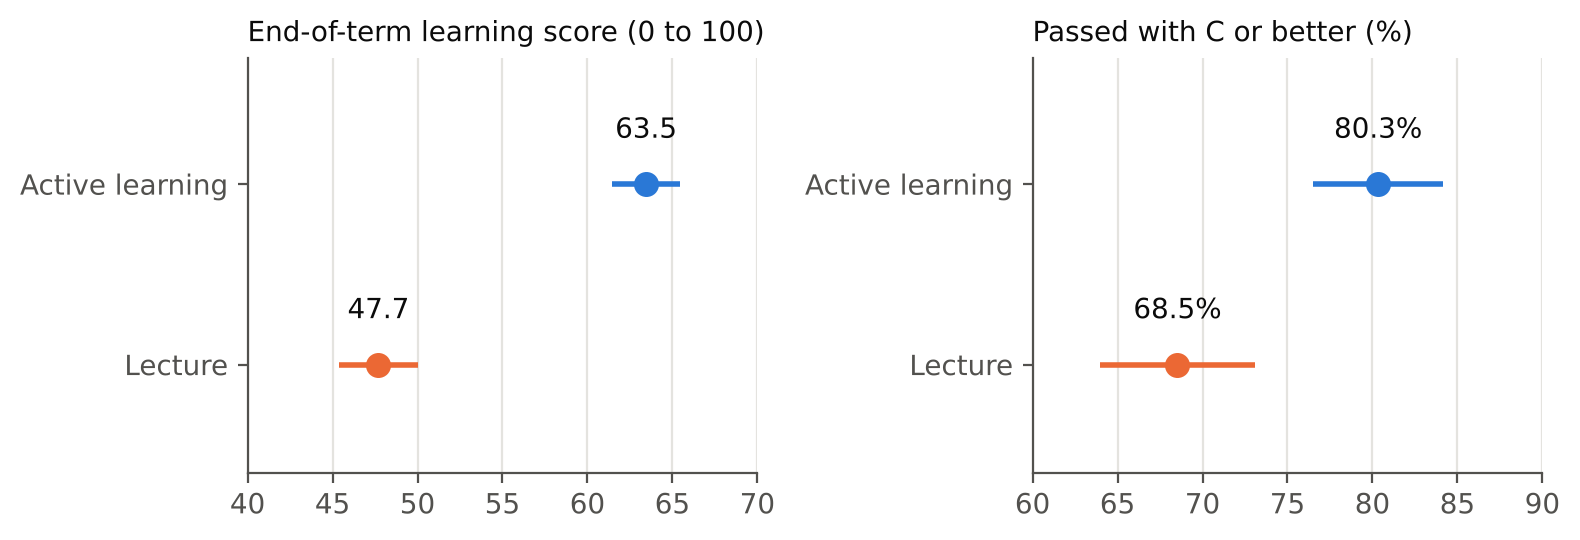
\includegraphics[width=0.86\textwidth]{figures/fig1_outcomes.png}
\caption{\textbf{Left:} Mean end-of-term learning measure by condition. \textbf{Right:} Share passing with a C or better. Students who remained in their assigned section; bars are simple 95\% confidence intervals. Clustered estimates are given in Table~\ref{tab:main}.}
\label{fig:outcomes}
\end{figure*}

\begin{table*}[t]
\centering
\caption{Outcomes and estimated effects of active learning}
\label{tab:main}
\begin{tabular}{lccl}
\toprule
Outcome & Active learning & Lecture & Estimated effect [95\% CI] \\
\midrule
Students in assigned section at drop/add & 417 & 394 & \nodata \\
Learning measure, mean (SD) & 63.5 (19.8) & 47.7 (21.0) & \\
\quad Time-slot fixed effects & & & 15.8 [11.8, 19.8] points \\
\quad Adding prior preparation & & & 16.3 [12.8, 19.7] points \\
\quad Hedges' $g$ & & & 0.77 [0.62, 0.93] \\
\quad Lee bounds for missing scores & & & 11.7 to 20.7 points \\
Passed with C or better & 80.3\% & 68.5\% & \\
\quad Time-slot fixed effects & & & 11.7 [6.4, 17.1] pp \\
\quad Adding prior preparation & & & 11.9 [6.8, 17.0] pp \\
D, F, or withdrawal (DFW) & 19.7\% & 31.5\% & 37.5\% relative reduction \\
\bottomrule
\end{tabular}
\tablecomments{Students who remained in their assigned section ($n = 811$). Effects are from ordinary least squares with time-slot fixed effects and standard errors clustered by section (32 clusters). pp = percentage points.}
\end{table*}


\subsection{Learning}\label{sec:learning}

Students in active-learning sections averaged \LMmeanAct\ on the end-of-term learning measure, compared with \LMmeanLec\ in lecture sections (Table~\ref{tab:main}; Figure~\ref{fig:outcomes}). Within time slots, the estimated effect was \LMest\ points (95\% CI \LMlo\ to \LMhi; \LMp), and \LMadj\ points after adjusting for prior preparation. The standardized effect was $g = \Gval$ (95\% CI \Glo\ to \Ghi).

The section-level analysis gave the same answer: the active section scored higher in \PairsFav\ of \PairsN\ slots, with a mean paired difference of \PairsMean\ points (exact randomization \PairsPexact; Figure~\ref{fig:pairs}; Table~\ref{tab:pairs} in Appendix~\ref{app:pairs}).

Lee bounds placed the learning effect between \LeeLo\ and \LeeHi\ points ($g$ between \LeeGlo\ and \LeeGhi). Even under the assumption most unfavorable to active learning, the benefit remained large. Consistent with selective missingness, lecture students without a score had lower prior preparation (\PrepNoScoreLec) than lecture students with one (\PrepScoreLec).

\begin{figure*}[t]
\centering
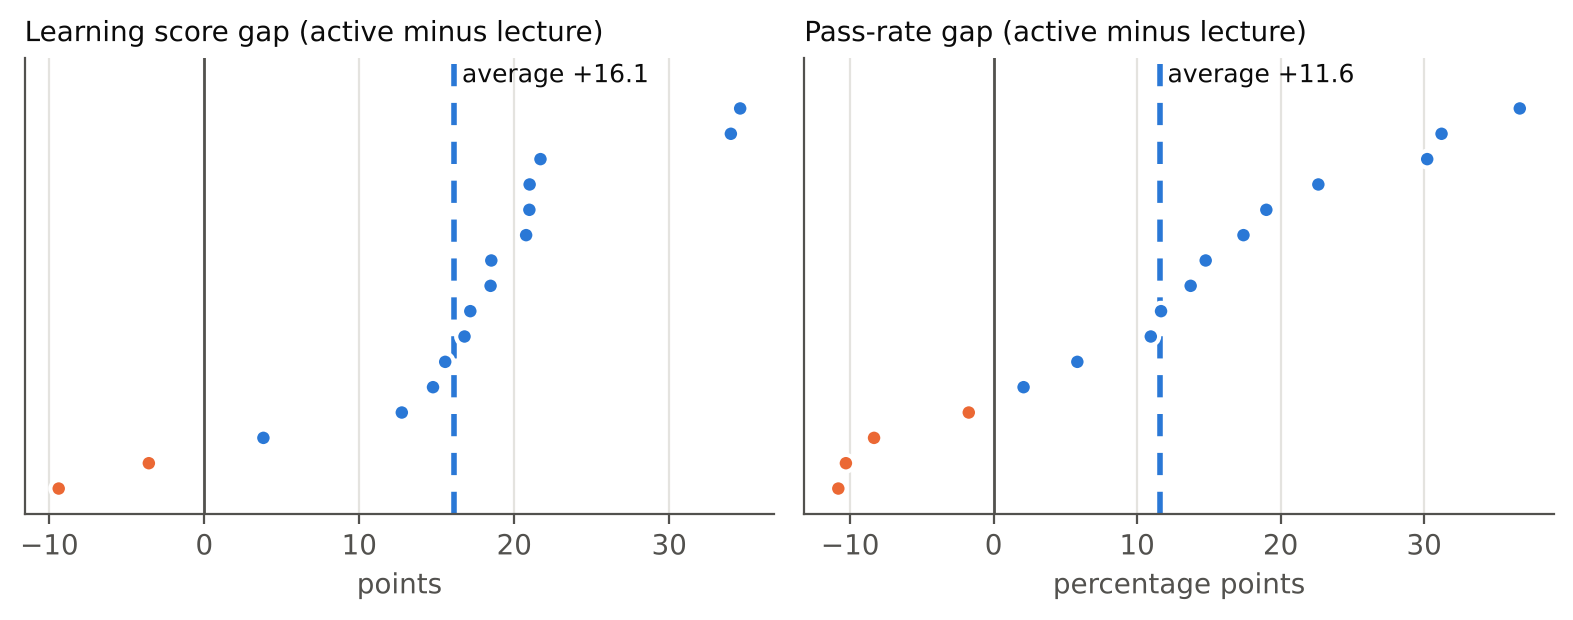
\includegraphics[width=0.86\textwidth]{figures/fig2_section_pairs.png}
\caption{Differences between the active-learning and lecture sections within each of the \PairsN\ registration time slots. \textbf{Left:} learning measure. \textbf{Right:} pass rate. The dashed line marks the mean difference; blue points favor active learning and orange points favor lecture.}
\label{fig:pairs}
\end{figure*}

\subsection{Passing and DFW Rates}\label{sec:passing}

\PassAct\ of active-learning students passed with a C or better, compared with \PassLec\ of lecture students. The within-slot effect was \PassEst\ percentage points (95\% CI \PassLo\ to \PassHi; \PassP) and was essentially unchanged by adjustment for prior preparation (\PassAdj\ points). Equivalently, the DFW rate fell from \DFWLec\ to \DFWAct, a \DFWRed\ relative reduction. At the section level, the active section had the higher pass rate in \PassPairsFav\ of \PairsN\ slots (exact randomization \PassPairsPexact).

\subsection{Student Groups}\label{sec:groups}

Gains on the learning measure were similar in every group examined, ranging from \SubLMmin\ to \SubLMmax\ points (Figure~\ref{fig:groups}; Table~\ref{tab:subgroups} in Appendix~\ref{app:groups}). Pass-rate gains were more variable, as expected with smaller samples, and were largest among Hispanic or Latino/a students (\SubPassHisp\ points) and transfer students (\SubPassTransfer\ points). Among Black or African American students ($n = \Nblack$), pass rates were \BlackPassAct\ under active learning and \BlackPassLec\ under lecture, a difference whose interval narrowly included zero. No condition-by-group interaction was statistically reliable (smallest $p = \MinInterP$), so the data do not show that any group benefited more or less than others.

\begin{figure*}[t]
\centering
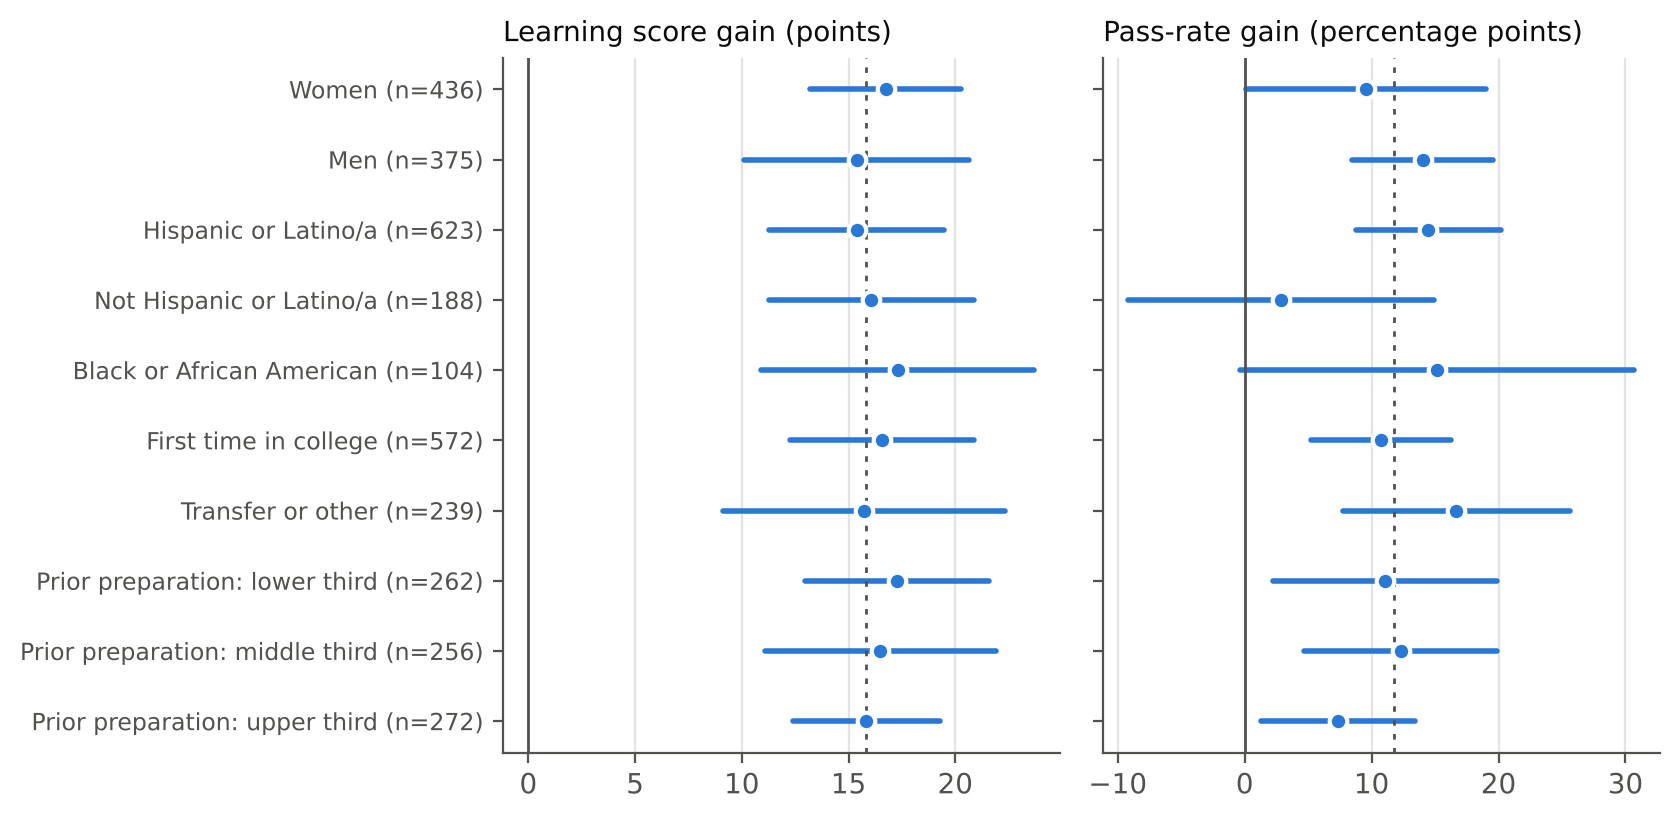
\includegraphics[width=0.86\textwidth]{figures/fig3_subgroups.png}
\caption{Estimated effects of active learning within student groups (exploratory). \textbf{Left:} learning measure. \textbf{Right:} pass rate. Lines are 95\% confidence intervals clustered by section; the dotted line is the whole-sample estimate.}
\label{fig:groups}
\end{figure*}

\section{Discussion}\label{sec:discussion}

Using only the public data and independent code, this re-analysis reproduced the central finding of \citet{kramer2023}: randomly allocated students in active-learning calculus sections learned substantially more than those in lecture sections. It adds three things. First, the benefit extends to course passing, the outcome that determines whether students continue in STEM: roughly \PerHundred\ more students per hundred passed. Second, the learning benefit survives a worst-case treatment of the trial's differential missing data. Third, the benefit appears broadly shared: at an institution where most students are Hispanic or Latino/a, active learning raised outcomes across gender, ethnicity, transfer status, and levels of prior preparation.

The size of the learning effect ($g \approx \Gval$) is larger than the average effects on examination scores in STEM-wide meta-analyses \citep{freeman2014}. Several features may contribute: a full curriculum redesign rather than added activities, a common learning measure designed for the study, and a comparison with lecture courses at a single institution. These same features limit generalization, which is why open data matter: other institutions can apply the same code to their own course records and test whether the effect replicates.

\section{Caveats}\label{sec:caveats}

Secondary analyses of a single trial carry their own limitations, and we want to be transparent about them. First, this is one trial at one institution, so results may not generalize to other student populations or curricula. Second, instructors were not crossed with conditions (\NinstrAct\ taught active sections and \NinstrLec\ taught lecture), so instructor differences cannot be fully separated from the teaching approach; clustering by section widens intervals to reflect this but does not remove it.

Third, course grades were assigned by instructors who knew the condition, so the pass-rate outcome is less standardized than the common learning measure. Fourth, the learning measure was missing more often in lecture sections; Lee bounds address this under a monotonicity assumption. Fifth, students who switched to non-trial sections have no outcomes, so estimates apply to students who remained in their assigned section. Sixth, subgroup analyses are exploratory. Finally, the data documentation reports three fewer active-learning students with a learning score than the file contains; this does not affect the conclusions.

\section{Conclusion}\label{sec:conclusion}

We re-analyzed the openly released data from a randomized trial of active learning in first-semester calculus, using independent code and a fully reproducible pipeline. We find four main conclusions.

\begin{itemize}
\item Active learning raised end-of-term learning by \LMest\ points on a 0--100 scale ($g = \Gval$), reproducing the central result of \citet{kramer2023} from the public data alone.
\item The benefit extends to course passing: \PassAct\ of active-learning students earned a C or better, compared with \PassLec\ of lecture students, and the DFW rate fell by \DFWRed.
\item The learning gain is robust to differential missing data, remaining at least \LeeLo\ points under worst-case Lee bounds, and appears in \PairsFav\ of \PairsN\ section pairs.
\item The benefit was similar across gender, ethnicity, transfer status, and prior preparation; no student group showed a reliably different effect.
\end{itemize}

Open, checkable evidence of this kind lets departments decide how to teach calculus with confidence. The next version of this project will place these results in national context by extracting the calculus and mathematics studies from published meta-analyses, and will invite departments to run the open pipeline on their own course records.

\vspace{6pt}
{\footnotesize
\noindent The author thanks Kramer, Fuller, Watson, Castillo, Duran Oliva, and Potvin for making their trial data openly available. This research received no funding. The author declares no competing interests. This study is a secondary analysis of fully anonymized, publicly released data and involved no contact with participants. Claude (Anthropic) assisted with writing analysis code, building figures, and drafting text; the author directed the analysis, checked every reported number against the data, and takes full responsibility for the content.

\vspace{4pt}
\noindent\textit{Data availability:} The original data are available from Dryad and Zenodo under CC0 \citep{kramer2023data}. All code, derived data, quality-check reports, and figures are available at \url{\RepoURL} and archived on Zenodo; the DOI is listed in the repository README.

\vspace{4pt}
\noindent\textit{Software:} pandas \citep{mckinney2010}, NumPy \citep{harris2020}, SciPy \citep{virtanen2020}, Matplotlib \citep{hunter2007}.\par}

\onecolumn
\appendix
\renewcommand{\thesection}{\Alph{section}}
\begin{center}APPENDIX\end{center}
\vspace{6pt}

\section{Section-Level Comparisons}\label{app:pairs}

Table~\ref{tab:pairs} lists the learning-measure and pass-rate comparisons for each of the \PairsN\ registration time slots that form the design-based check in Section~\ref{sec:learning}. Each slot contained one active-learning section and one lecture section, so these comparisons hold the time of day and day of week fixed.

\begin{table}[h!]
\centering\small\setlength{\tabcolsep}{5pt}
\caption{Section-level comparison within each registration time slot}
\label{tab:pairs}
\begin{tabular}{cccccccc}
\toprule
& \multicolumn{2}{c}{$n$ with score} & \multicolumn{2}{c}{Mean learning score} & & \multicolumn{2}{c}{Pass rate} \\
\cmidrule(lr){2-3}\cmidrule(lr){4-5}\cmidrule(lr){7-8}
Slot & Active & Lecture & Active & Lecture & Difference & Active & Lecture \\
\midrule
1 & 28 & 20 & 71.3 & 52.8 & +18.5 & 78.1\% & 60.7\% \\
2 & 29 & 21 & 54.9 & 64.3 & $-$9.4 & 86.2\% & 71.4\% \\
3 & 26 & 22 & 68.7 & 47.7 & +21.0 & 66.7\% & 75.0\% \\
4 & 17 & 20 & 61.7 & 27.1 & +34.6 & 61.9\% & 63.6\% \\
5 & 23 & 18 & 51.1 & 54.7 & $-$3.6 & 95.8\% & 90.0\% \\
6 & 29 & 22 & 58.1 & 45.3 & +12.7 & 93.5\% & 63.3\% \\
7 & 17 & 11 & 61.6 & 57.8 & +3.8 & 88.2\% & 69.2\% \\
8 & 14 & 8 & 53.3 & 19.3 & +34.0 & 86.7\% & 50.0\% \\
9 & 26 & 25 & 68.5 & 53.8 & +14.8 & 60.6\% & 71.4\% \\
10 & 30 & 29 & 66.2 & 45.5 & +20.8 & 87.1\% & 55.9\% \\
11 & 29 & 24 & 71.2 & 54.0 & +17.2 & 76.7\% & 65.7\% \\
12 & 29 & 21 & 58.4 & 39.9 & +18.5 & 81.2\% & 58.6\% \\
13 & 34 & 31 & 64.7 & 43.0 & +21.7 & 94.3\% & 80.6\% \\
14 & 22 & 20 & 74.3 & 53.3 & +21.0 & 76.0\% & 73.9\% \\
15 & 12 & 9 & 61.1 & 44.3 & +16.8 & 86.7\% & 75.0\% \\
16 & 11 & 9 & 62.0 & 46.5 & +15.5 & 64.7\% & 75.0\% \\
\bottomrule
\end{tabular}
\tablecomments{Each slot contained one active-learning section and one lecture section. Score columns use students with a learning measure; pass columns use all students who remained in the section.}
\end{table}


\section{Student-Group Estimates}\label{app:groups}

Table~\ref{tab:subgroups} gives the numerical estimates plotted in Figure~\ref{fig:groups}. All estimates are exploratory and should be read together with the interaction tests in Section~\ref{sec:groups}.

\begin{table}[h!]
\centering\small\setlength{\tabcolsep}{5pt}
\caption{Effects of active learning within student groups (exploratory)}
\label{tab:subgroups}
\begin{tabular}{lccccc}
\toprule
Group & $n$ & Learning gain & Pass rate, & Pass rate, & Pass-rate gain, \\
 & & points [95\% CI] & active & lecture & pp [95\% CI] \\
\midrule
Women & 436 & 16.7 [13.2, 20.3] & 79.0\% & 69.0\% & 9.5 [0.1, 19.0] \\
Men & 375 & 15.4 [10.1, 20.7] & 82.1\% & 68.1\% & 14.0 [8.5, 19.6] \\
Hispanic or Latino/a & 623 & 15.4 [11.3, 19.5] & 82.6\% & 68.2\% & 14.5 [8.7, 20.2] \\
Not Hispanic or Latino/a & 188 & 16.1 [11.3, 20.9] & 72.9\% & 69.6\% & 2.9 [$-$9.2, 14.9] \\
Black or African American & 104 & 17.3 [10.9, 23.7] & 70.0\% & 51.9\% & 15.2 [$-$0.3, 30.7] \\
First time in college & 572 & 16.6 [12.3, 20.9] & 83.5\% & 72.6\% & 10.7 [5.2, 16.3] \\
Transfer or other & 239 & 15.7 [9.1, 22.3] & 73.0\% & 58.4\% & 16.7 [7.7, 25.6] \\
Prior preparation, lower third & 262 & 17.3 [13.0, 21.6] & 68.9\% & 56.7\% & 11.1 [2.2, 19.9] \\
Prior preparation, middle third & 256 & 16.5 [11.1, 21.9] & 81.3\% & 70.1\% & 12.3 [4.7, 19.9] \\
Prior preparation, upper third & 272 & 15.8 [12.4, 19.3] & 90.4\% & 82.5\% & 7.3 [1.3, 13.4] \\
\bottomrule
\end{tabular}
\tablecomments{Estimates from ordinary least squares with time-slot fixed effects within each group; confidence intervals clustered by section. Groups overlap and are not mutually exclusive.}
\end{table}


\clearpage
\twocolumn
\begin{center}REFERENCES\end{center}
\vspace{4pt}
{\footnotesize
\renewcommand{\section}[2]{}%
\begin{thebibliography}{99}
\setlength{\itemsep}{1pt}
\bibitem[Bressoud et~al.(2015)]{bressoud2015}
Bressoud, D., Mesa, V., \& Rasmussen, C., eds. 2015, Insights and Recommendations from the MAA National Study of College Calculus (Washington, DC: MAA Press)

\bibitem[Cameron \& Miller(2015)]{cameron2015}
Cameron, A.~C., \& Miller, D.~L. 2015, Journal of Human Resources, 50, 317, doi:~\href{https://doi.org/10.3368/jhr.50.2.317}{10.3368/jhr.50.2.317}

\bibitem[Freeman et~al.(2014)]{freeman2014}
Freeman, S., Eddy, S.~L., McDonough, M., et~al. 2014, Proceedings of the National Academy of Sciences, 111, 8410, doi:~\href{https://doi.org/10.1073/pnas.1319030111}{10.1073/pnas.1319030111}

\bibitem[Harris et~al.(2020)]{harris2020}
Harris, C.~R., Millman, K.~J., van~der Walt, S.~J., et~al. 2020, Nature, 585, 357, doi:~\href{https://doi.org/10.1038/s41586-020-2649-2}{10.1038/s41586-020-2649-2}

\bibitem[Hedges(1981)]{hedges1981}
Hedges, L.~V. 1981, Journal of Educational Statistics, 6, 107, doi:~\href{https://doi.org/10.3102/10769986006002107}{10.3102/10769986006002107}

\bibitem[Hunter(2007)]{hunter2007}
Hunter, J.~D. 2007, Computing in Science \& Engineering, 9, 90, doi:~\href{https://doi.org/10.1109/MCSE.2007.55}{10.1109/MCSE.2007.55}

\bibitem[Kramer et~al.(2023a)]{kramer2023}
Kramer, L., Fuller, E., Watson, C., et~al. 2023a, Science, doi:~\href{https://doi.org/10.1126/science.ade9803}{10.1126/science.ade9803}

\bibitem[Kramer et~al.(2023b)]{kramer2023data}
Kramer, L., Fuller, E., Watson, C., et~al. 2023b, Establishing a New Standard of Care for Calculus Using Trials with Randomized Student Allocation [Dataset], Dryad, doi:~\href{https://doi.org/10.5061/dryad.kkwh70s95}{10.5061/dryad.kkwh70s95}

\bibitem[Laursen et~al.(2014)]{laursen2014}
Laursen, S.~L., Hassi, M.-L., Kogan, M., \& Weston, T.~J. 2014, Journal for Research in Mathematics Education, 45, 406, doi:~\href{https://doi.org/10.5951/jresematheduc.45.4.0406}{10.5951/jresematheduc.45.4.0406}

\bibitem[Lee(2009)]{lee2009}
Lee, D.~S. 2009, Review of Economic Studies, 76, 1071, doi:~\href{https://doi.org/10.1111/j.1467-937X.2009.00536.x}{10.1111/j.1467-937X.2009.00536.x}

\bibitem[McKinney(2010)]{mckinney2010}
McKinney, W. 2010, in Proceedings of the 9th Python in Science Conference, 56, doi:~\href{https://doi.org/10.25080/Majora-92bf1922-00a}{10.25080/Majora-92bf1922-00a}

\bibitem[Springer et~al.(1999)]{springer1999}
Springer, L., Stanne, M.~E., \& Donovan, S.~S. 1999, Review of Educational Research, 69, 21, doi:~\href{https://doi.org/10.3102/00346543069001021}{10.3102/00346543069001021}

\bibitem[Theobald et~al.(2020)]{theobald2020}
Theobald, E.~J., Hill, M.~J., Tran, E., et~al. 2020, Proceedings of the National Academy of Sciences, 117, 6476, doi:~\href{https://doi.org/10.1073/pnas.1916903117}{10.1073/pnas.1916903117}

\bibitem[Virtanen et~al.(2020)]{virtanen2020}
Virtanen, P., Gommers, R., Oliphant, T.~E., et~al. 2020, Nature Methods, 17, 261, doi:~\href{https://doi.org/10.1038/s41592-019-0686-2}{10.1038/s41592-019-0686-2}
\end{thebibliography}}

\end{document}
